\section{Self Power Modeling Methodology}
\label{sec:method}

In this section, we first describe the basic self power modeling
methodology. We then discuss a set of practical challenges in applying
SPMD  and how we address them:
(1) How to set up the system of equations?
(2) How to constrain the solver to make it output meaningful models?
(3) How to validate the SPMD-derive models?
(4) Are built-in power sensors accurate enough for use in SPMD?

\if 0
present a set of constraints that we add to the
basic solver to help the solver to output meaningful model parameters.
and for the usabiity of Android phones power sensor readings.
\fi

% as depicted in Figure~\ref{fig:equations}.
\if 0
\begin{figure}[tp]
    \centering
    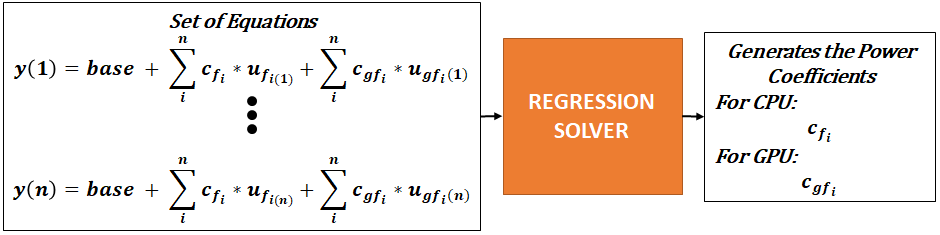
\includegraphics[width=0.95\columnwidth]{figures/design_2.png}
    \vspace{-0.1in}
    \caption{SPMD via solving a system of linear equations.}
    \label{fig:equations}
    \vspace{-0.1in}
\end{figure}
\fi

\begin{table}[t]
{\footnotesize
    \centering
    \caption{Power state, utilization, and energy collected during online app run.}
    \vspace{-0.1in}
   % \begin{tabular}{|p{32mm}|p{10mm}|p{23mm}|}
    \begin{tabular}{|l|P{11mm}|c|}
    \hline
          &  Symbol & Collection method \\
         \hline
         \multicolumn{1}{|l|}{\textbf{Power State}} &  &   \\
         CPU Frequency      & $f_{k}$                               & cpu\_frequency \\
         GPU Frequency      & $g_{k}$                               & kgsl\_pwrlevel \\
         GPU State          & $s_j$                                 & kgsl\_pwr\_set\_state \\
         \hline
          \multicolumn{1}{|l|}{\textbf{Utilization}} &   &  \\
         
         \multicolumn{1}{|l|}{CPU Util. in freq. $f_k$}               & $u^c(f_{k})$        & cpu\_idle \\
         \multicolumn{1}{|l|}{GPU Util. in freq. $g_k$,}  & $u^g(g_k,s_j)$      & kgsl\_pwrstats \\
          \mbox{\hspace{0.6in}}state $s_j$ & & \\
         \hline
         \multicolumn{1}{|l|}{Energy drain}     & $y$                                &
         \multicolumn{1}{p{30mm}|}{/sys/class/power\_supply /charge\_counter} \\
         \hline
    \end{tabular}
    \label{tab:triggers}
    \vspace{-0.2in}
}
\end{table}

\subsection{Basic SPMD Process}
\label{subsec:generic}

As discussed in \S\ref{subsec:spmd}, SPMD consists of two basic steps: 
\dcomment{(1)} online data collection for setting up a system of equations and 
\dcomment{(2)} offline model derivation by solving the system of equations.

\paragraph{Online data collection.}
Since SPMD is "in-situ", we need to collect the data needed to set up the
equations while the app is running.
% As discussed in \S\ref{sec:primer}, in modern phones, the CPU and GPU power draw are 
% functions of the operating frequency and the power state (for GPU). Therefore,
% for power triggers, we need to collect the duration each component spends in every 
% combination of frequency and power-state during the app run, as listed in Table~\ref{tab:triggers}.
%
Table~\ref{tab:triggers} lists the data that need to be collected and
how they are collected on Android phones.  The data include the power
states and utilization in each state of each component used by the
app,
%  for each time interval corresponding to an equation 
as well as the whole-phone power draw or energy drain,
\eg in every small time interval during app run.

We use the Linux event trace~\cite{eventtrace} to collect the power
state and utilization.  To collect whole-phone energy draw per
time interval, we can use either the built-in power sensor energy counter
which became available since Android {7}, or an external power
monitor such as Monsoon~\cite{monsoonpowermonitor}.

\cut{ Ideally, reading from the built-in power sensor is preferred,
  since it does not require wiring the phone battery and potentially
  allows SPMD to be performed on any phones, including users' phones
  "in the wild". However, as we will see in the next section, built-in
  power sensor readings have such high error that makes them
  impractical to use in SPMD.  }

\if 0
\begin{figure}[tp]
{\small
    \centering
    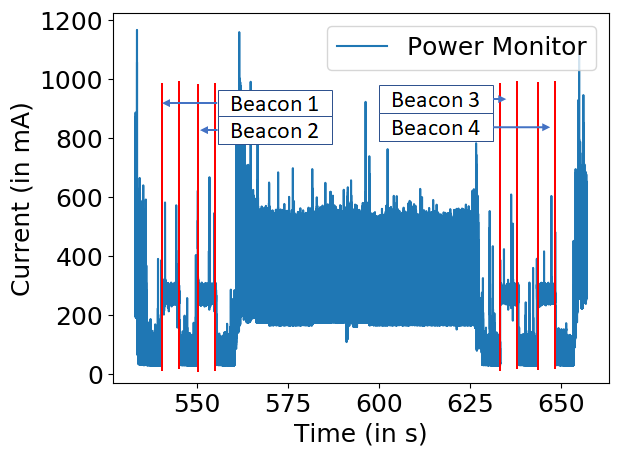
\includegraphics[width=0.80\columnwidth]{figures/beacons_3.png}
    \vspace{-0.1in}
    \caption{Beacons to align power monitor with phone clock.}
    \label{fig:align_beacon}
    \vspace{-0.1in}
}
\end{figure}
\fi

%%%%%%%%%%%%%%%
\paragraph{Offline model derivation.} 
%
% In offline processing, \eg 
When the app run finishes, SPMD sets up a system of linear
equations with the phone component power parameters as unknowns.  In
general, the trace duration is cut into $K$ equal intervals of $T$
seconds each, and one equation is created for interval $t$ as follows:
\begin{align}
y_t = p^{c}_{\text{base}} +& \sum_i\sum_k{u^c_t(f_k)p_i^{c}(f_{k})} + \nonumber \\
        & \sum_{j}\sum_{k} u^g_t(g_k,s_j)p^{g}(g_k, s_j)
\end{align}
where the double summation for the CPU is over all the CPU cores and frequencies,
the double summation for the GPU is over all the GPU frequencies and GPU states,
$u^c_t(f_k)$ and $u^g_t(g_k,s_j)$ are the CPU and GPU utilization for the corresponding power states
in time interval $k$,
and the left-hand-side (LHS) $y_t$ is the total phone energy drain in time interval $t$.
% where model parameter $p^c(f_{i})$ is the CPU power draw for frequency $f_i$,  
% model parameter $p^g_{ij}$ is the GPU power draw at frequency $f_i$ and power state $j$, the utilization coefficients $_{f_{i}}(k)$ and $u_{ij}(k)$ equal the total utilization (in seconds) of CPU and GPU in the corresponding frequencies and power states in the $k$th trace interval, and $y(k)$ denotes the total phone energy drain during interval $k$ from integrating power sensor or power monitor readings.
% \cut{ 
% Clearly, in a given app run, the CPU and GPU may not go through all possible frequencies and power states, and hence not all power parameters may show up in the equations. SPMD will only derive those power model
% parameters actually encountered in the app run. This is not an issue with SPMD as only those parameters will be needed for the power model applications such as energy profiling or energy debugging. 
% }
\st{Since there can be more equations than the number of unknowns, 
the system of equations can be solved using a regression-based
solver to generate the power parameters.} In this paper, we use
the python curve\_fit() function which uses {\color{blue}the}
\dcomment{non-linear}
least square fitting as our regression solver~\cite{curvefit}.

Notice that although SPMD via solving a system of equations using a regression solver is
conceptually simple{\color{blue}, due to the existence of noise in measurement, the modeling results from linear regression solver could be invalid. Further, different setup will affect the final modeling results. Therefore, it is worthwhile to examine the modeling quality of SPMD under different settings and understand why SPMD works or not with certain setup.}

\if 0
\subsection{SPMD Challenges}
\label{subsec:challenges}

SPMD via solving a system of equations using a regression solver is conceptually simple. 
In practice, the single biggest challenge is whether the system of equations 
has enough diversity so that the regression solver
can generate meaningful solutions to the system, \ie power model parameters. 
The answer is not obvious for at least two reasons.

{\bf Condition 1: Usage coefficients lack diversity.}
First, \S\ref{sec:primer} has concluded that
we need to set up a system of equations for each app scenario as different scenarios
even of the same app can have different component usage. However, 
one can imagine that the app behavior for the same app scenario may be highly repetitive and hence
the resulting equations, either the usage terms on one side or the energy drain on the other side,
 may look similar or only differ slightly, resulting on low rank of the equations. 

{\bf Condition 2:s Noisy energy measurement.}
The energy measurement can contain noise and if the difference among the true energy values for different equations is small, the noise level may dominate the energy variations of the different equations. This can result in the regression solver trying to minimize the fitting error from noisy energy measurement as opposed to fitting the true energy difference.  

Our verification study centers around addressing this challenge, by systematically exploring different ways of setting the system of equations to try to increase the diversity.

Before presenting our verification study, we discuss two refinements we added
to the basic SPMD methodology.


\fi

\subsection{How to Set up Equations?}
\label{subsec:howtosetup}

The basic SPMD methodology does not specify how to set up systems of
equations for the regression solver for a given app run. Since SPMD is
"in-situ", \ie it derives all the power model parameters experienced
during a given app run, in principle we need to create equations that
cover the entire app run duration.  Given an app run of duration
$T$, we can potentially chop it into $N_s$ equal-sized epochs, and
set up $N_e$ equations per each epoch, each covering a duration of
$t_e$ of the app run, \ie
\begin{eqnarray}
T = N_s \cdot N_e \cdot t_e
\end{eqnarray}
%
Thus, setting equations for SPMD has two degrees of freedom: 
(1) How many systems of equations $N_s$ shall we create for an app run? 
(2) How many equations $N_e$ shall we create for each epoch?
Our verification study explores how the two degrees of freedom can 
help us \st{to improve the diversity for the systems of equations.}{\color{blue} to get valid modeling results.}

\subsection{Adding Constraints to the Solver}
\label{subsec:constraint}

As we will see in \S\ref{sec:modelling_macro}, because the regression
solver tries to minimize the fitting error and is oblivious to the
semantics of the unknowns, it may output solutions that minimize the
fitting error but violate basic properties of the power model
parameter values, such as non-negativity {\color{blue}(all coefficients should not be negative)} and monotonicity {\color{blue}(coefficients of higher frequency should be larger)}.  To overcome
this, in addition to the basic unconstrained regression solver, {\color{blue}we also experimented two constrained regression solver} based on the domain knowledge of power models, as shown in
Table~\ref{tab:constrained}.

\begin{table}[tp]
%\questionaj{These constraints must also constrain GPU busy and idle.}
{\small
    \centering
    \caption{Constraints added to the regression solver.}
    \vspace{-0.1in}
    \begin{tabular}{|p{25mm}|p{52mm}|}
    \hline
         Constrained SPMD  & \multicolumn{1}{c|}{Description} \\
         \hline
\hline
         Unconstrained      & No constraints are applied. \\
\hline
         Constrained        & Model parameters should not decrease with increasing frequencies. GPU idle power is less than GPU busy power. \\
\hline
         Freq-constrained   & CPU model parameters are modeled as a polynomial of frequency. \\
         \hline
    \end{tabular}
    \label{tab:constrained}
    \vspace{-0.1in}
}
\end{table}


\paragraph{Constraint 1: positivity and monotonicity.}
Without any constraint, we found the regression solver can output
CPU/GPU power values that are negative or decreasing when the
frequency increases.  To prevent the solver from outputing such
solutions, we added three constraints to the regression solver: (1) all
model parameters should be positive; (2) the model parameters with
increasing frequencies for each component should be non-decreasing;
(3) the GPU Idle power should be lower than the GPU Busy power.  We
denote this version of SPMD as "Constrained SPMD".


\paragraph{Constraint 2: modeling CPU power as a function of frequency.}
We found even with Constraint 1, the CPU power parameters with varying
frequencies output by the solver often remain the same.  To make the
CPU model parameters output more consistent with the reality, we
exploited another domain knowledge about the CPU power draw, that it
increases as a low-order polynomial of the operating
frequency~\cite{armdvfs,rizvandi2011some}.
% Since the specific polynomial function may vary for different phones, \eg early phones only performed % frequency scaling (FS) while newer phones perform dynamic voltage and frequency scaling (DVFS), we first used a simple CPU benchmark to find the order of the polynomial for each phone used in our experiments. 
%
\if 0
\begin{figure}[tp]
    \centering
%    \vspace{-0.1in}
    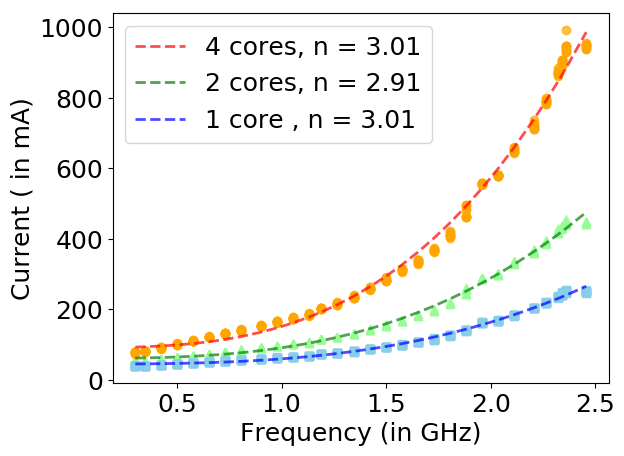
\includegraphics[width=0.80\columnwidth]{figures/cpu_characteristics.png}
    \caption{Moto Z3 big core CPU power draw grows with frequency 
    when running the arithmetic-intensive benchmark.}
    \label{fig:cpu_characteristic}
    \vspace{-0.1in}
\end{figure}
\fi
%
\cut{ We ran a microbenchmark that performs arithmetic-intensive or memory-intensive operations for 7 seconds
on 1, 2 and 4 big cores, for each big core frequency, and fit the measured phone power 
with a polynomial function in frequency.
%\begin{equation}
%     P_{CPU} = p^c_{base}+ \sum_i p^c_i({f_k}) = p_{base}+\sum_i  a*f_k^{n}
% \end{equation}
% Figure~\ref{fig:cpu_characteristic} shows the measured power draw and curve fitting on Moto Z3.
}
Our CPU microbenchmark results show  that 
% the fitted exponent $n$ for 1, 2 and 4 cores are 3.01, 2.97 and 3.01, respectively.
the per-core power grows as the third-power of the CPU
frequency on all three phones, 
\ie $p_i^c(f_k) = a\cdot f_k^3$. 
Thus we replace all the CPU power parameters with
third-power of the CPU frequency in the SPMD model equations.
%model the Moto Z3 big core power as a third-order polynomial of the CPU frequency in the model equations of SPMD.
%
Doing so has two benefits: (1) it reduces the number of CPU power
parameters from $K$, the number of CPU frequencies, to 2, the base power $p_{\text{base}}$
and coefficient $a$, which reduces the number of equations needed for
the solver; (2) it constraints the CPU power to be not only
monotonically increasing with its frequency, but also consistent with its physical power behavior.


%%%%%%%
\subsection{How to Validate Modeling Results from SPMD?}
\label{subsec:validate}

{\color{blue}Because SPMD aims to generate different modeling results for different scenarios, it is unreasonable to use measurements from other app runs to test our modeling results for a specific app run. However, since we have already assume that the ground truth is a linear model, we only need to verify that whether the output of the linear regression is validate or not. In the field of statistical learning, F-test and $R^2$-measurement are commonly used to validate the effectiveness of linear regression results. We thus use F-test and $R^2$-measurement as the quantitative validation on the SPMD modeling results.}

{\color{blue}Besides the statistical methods of validation, we will also check the modeling results qualitatively by the following standards:}
(1) {\em The trend of the model parameters derived should appear similar to
the model derived using TPMD}. For example, they should be positive,
follow monotonicity (\eg CPU power should grow with higher frequency),
and the GPU Idle power should be less than the GPU Busy power;
%
(2) {\em The specific values of the parameters should be within a threshold
of their counterparts in the TPMD derived model
parameters}. The threshold could be based on empirical evidence, \eg
from the power state variation study in \S\ref{sec:primer}.

\st{
Since the motivation of SPMD is to capture the power model's dependence on
app usage, SPMD is fundamentally different from 
TPMD.  As in conventional learning,
the goal of TPMD is to train a model based on training data from
some app run that will predict well the testing data for different
app runs.
%    and hence has to be concerned with over-fitting during training.
In contrast, the goal of SPMD is to generate the power model that
best fits the power draw of a given app run and not used for other app runs.
% , where overfitting is not an issue.
However, this also raises a fundamental challenge of how to
validate the derived model as we generally do not have the
ground-truth power model for a given app run.}

% In our study, we apply a three-pronged criteria to
% determine whether the derived SPMD model is considered acceptable:
% %
% (1) {\em The trend of the model parameters derived should appear similar to
% the model derived using TPMD}. For example, they should be positive,
% follow monotonicity (\eg CPU power should grow with higher frequency),
% and the GPU Idle power should be less than the GPU Busy power;
% %
% (2) {\em The specific values of the parameters should be within a threshold
% of their counterparts in the TPMD derived model
% parameters}. The threshold could be based on empirical evidence, \eg
% from the power state variation study in \S\ref{sec:primer}.
% %
% (3) {\em We apply conventional training-testing validation} by extracting
% interleaved training and testing data in a given app run to compare
% the fitting error for the training and testing data.  

\subsection{Can Power Sensor Readings be Used?}
\label{subsec:modelling_sensor}

Since using the built-in power sensor readings would allow SPMD to be
performed on any phone in the wild, we assess the feasibility of using
the power sensors in modern smartphones for developing SPMD, by
measuring the accuracy of their energy counter readings.

%{\bf Methodology }
%% 2. Explanation of equation generation
% Since in principle, the energy counter gives more accurate energy estimation for an equation interval than averaging all the instantaneous power readings in the interval multiplied by the interval duration,
% we use energy counter readings to generate the LHD of each model equation.
\begin{sloppy}
% The Android versions on both phones exports APIs for power sensor readings with
Android 7.0 and later versions provide 
interfaces to the built-in power sensor through sysfs~\cite{linuxsysfs} with
a finite sampling resolution, 1.4s on Pixel 2 and Moto Z3, and 380ms on Pixel 4.
{The power sensor readings have two formats}: instantaneous power draw 
({\small /sys/\-class/\-power\_supply/\-battery/\-current\_now}) and
energy counter ({\small /sys/\-class/\-power\_supply/\-battery/\-charge\_counter})
which reports the total energy in the previous sampling interval.
\end{sloppy}

We measured the accuracy of the Android energy counter reading by
comparing it with the readings from a
high-fidelity external Monsoon power monitor,
using a 250-second run of the YouTube app while the device is
connected to the power monitor.  We chose YouTube as it is a popular
app and exhibits significant power variations during its run.

\begin{figure}[tp]
    \centering
\if 0
\begin{subfigure}[b]{0.50\textwidth}
         \centering
         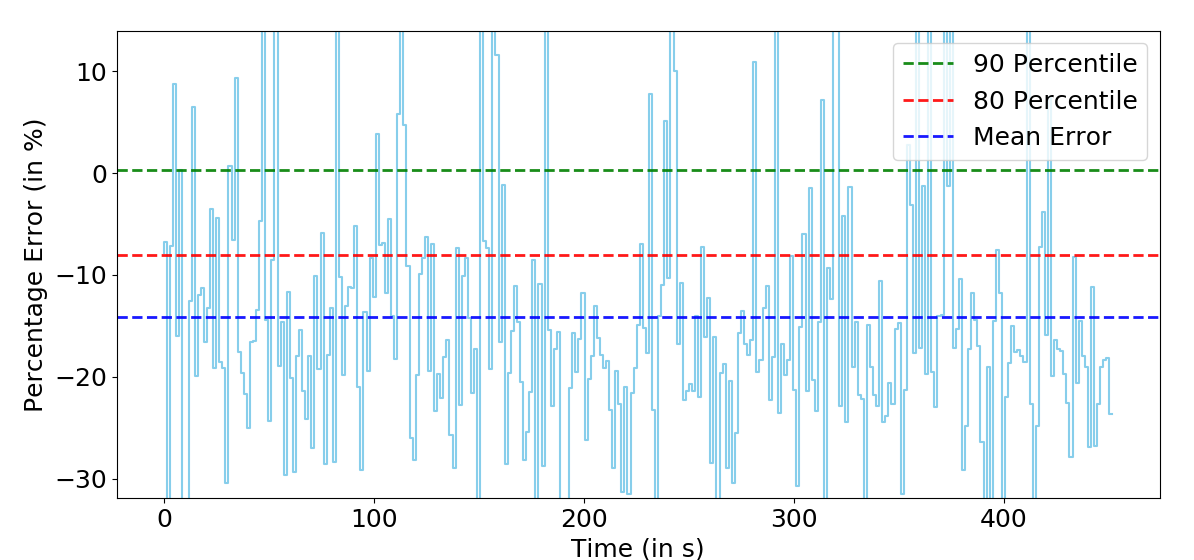
\includegraphics[width=\textwidth]{figures/sensor_error_timeline_5.png}
         \caption{Timeline on Moto Z3}
         \label{fig:sensor_error_timeline}
     \end{subfigure}
     \hfill
\fi

\begin{minipage}{0.48\columnwidth}
\begin{subfigure}[b]{\textwidth}
         \centering
         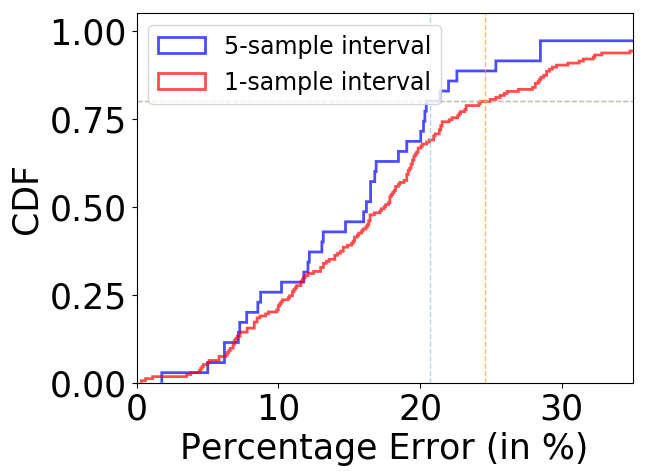
\includegraphics[width=\textwidth]{figures/sensor_error_cdf.png}
         % \caption{CDF for Moto Z3}
%         \label{fig:sensor_error_cdf_motoz3}
     \end{subfigure}
     
  \if 0
  \begin{subfigure}[b]{0.46\columnwidth}
         \centering
         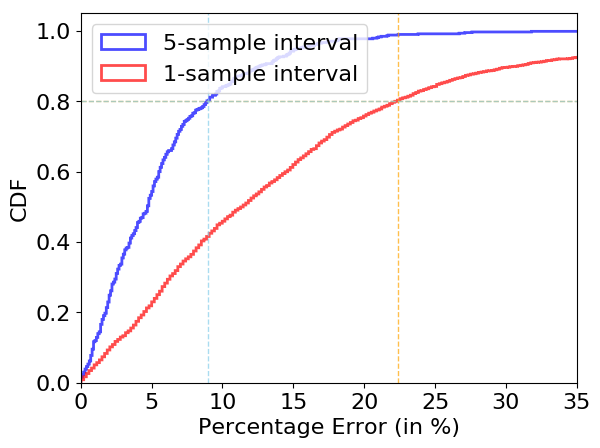
\includegraphics[width=\textwidth]{figures/sensor_error_cdf_nexus6.png}
         \caption{CDF for Nexus 6}
         \label{fig:sensor_error_cdf_nexus6}
     \end{subfigure}
  \fi
  \caption{Power sensor reading error relative to power monitor reading
        for the YouTube for Moto Z3.
        % In CDF, the orange line represents the 80 percentage for 1 sample and blue line represents for 5 sample
        }
        \label{fig:sensor_error}
        \vspace{-0.1in}
\end{minipage}
\hfill
\begin{minipage}{0.48\columnwidth}

    \centering
    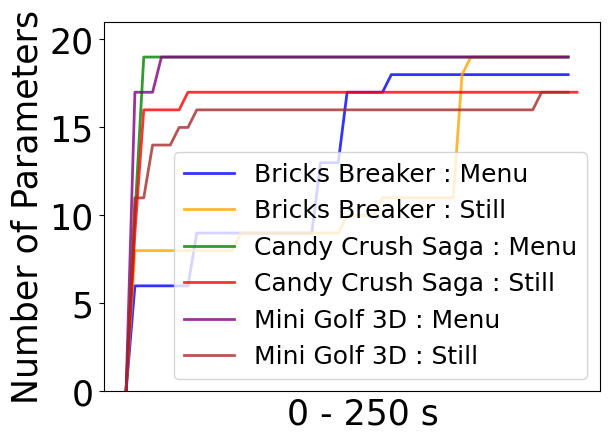
\includegraphics[width=\textwidth]{figures/004_Pixel4_cummulative_macro_parameters.png}
    \vspace{-0.1in}
    \caption{The cumulative number of unique parameters over app run duration on Pixel 4.}
    \label{fig:number_parameters_vs_duration}
    \vspace{-0.1in}
\end{minipage}
\end{figure}


 

%{\bf Findings}
%% 3. Explain power sensor is effects the accuracy of the equations
%Figure~\ref{fig:sensor_error} shows the timeline and the CDF for the sensor error.
\if 0
Figure~\ref{fig:sensor_error_timeline} shows the percentage error of the estimated energy
for 1-sample intervals (1.4s) based on power sensor reading over the 500s app run for Moto Z3.
We observe that \comment{for 89.7\% of the intervals the power sensor reading underestimates the energy drain compared to the power monitor reading.}
\fi

Figure~\ref{fig:sensor_error} shows the CDF for the absolute
percentage error on Moto Z3 for 1-sample (1.4s) and for 5-sample (7s)
intervals.  We plot the error for 5-sample intervals to see if
averaging over 5 samples can reduce the power sensor reading error.
% since if so we can set up an equation for each 5-sample interval as opposed to each 1-sample interval.
Figure~\ref{fig:sensor_error} shows
that the average error for 5-sample intervals, 15.84\%,
is only slightly better than that for 1-sample intervals, 19.01\%.
Similarly, the 80th percentile errors for 1-sample and 5-sample intervals
are 20.52\% and 24.18\% and median errors are 
16.76\% and 17.99\%, respectively.

\if 0
% , and the 80th percentile errors are 24.03\% and 21.10\%, respectively.
% Nexus 6
Figure~\ref{fig:sensor_error_cdf_nexus6} shows the CDF for the absolute percentage error
for 1-sample intervals (175 ms) and for 5-sample intervals (875 ms) for Nexus 6.
However, we see that the average error for 5-sample intervals, 7.21\%,
is lower than for 1-sample intervals of 19.06\%, and
the 80th percentile errors are 9.89\% and 26.60\%, respectively.
\comment{We observe that the sensor is about 3 times lower in Nexus 6 as compared to Moto Z3
for 1 sample interval is due to the interval of Nexus 6 being 8 times shorter than Moto Z3.
Suggesting that the low sampling rate of the sensor is the cause of the error.}
\fi
Such high error 
suggests that the built-in power sensor readings available on today's Android phones 
are not suitable for self power model derivation. 
Thus we conduct our SPMD study by using an external
Monsoon power monitor to generate the power draw ground truth.

\if 0
{\bf Reason }
%% 5. Reasons for the inaccuracies in power sensor
The high inaccuracy of the power sensor could be attributed to mainly 2 reasons.
\begin{itemize}
    \item {\bf Noise: } The power management circuit and it's location in the device is susceptible to noise due to the electronic circuitry involved in it.
    It can be argued that, the noise can be reduced by taking a longer interval which might average out the effect of noise, but from our finding we find that this approach is not effective.
    
    \item {\bf Low Sampling rate: } The power sensor generate a new value every 1.4 seconds interval in moto Z3.
    This greatly inhabits use of the power sensor to gather instantaneous current. 
 \end{itemize}
\fi


% The Monsoon power monitor has a sampling rate of 5 KHz  and has been widely used as the ground truth in smartphone power modeling and energy drain studies. 


\subsection{Aligning Power Monitor with Linux event trace}
\label{subsec:align}

As in TPMD, using an external power monitor in SPMD faces the challenge
of aligning the power monitor reading trace with the power event trace
logged on the phone, as the power monitor has a separate clock and
thus clock drifts from that of the phone. Accurate alignment is
critical to post-processing of SPMD as it directly affects how well the
two sides of each equation in the system of equations capture the same
time interval.

We achieve accurate trace alignment in two steps.  First, we run a
``beacon'' microbenchmark consisting of a 5-second CPU burst, and
align the time of the CPU utilization surge in the event trace with
the time of the corresponding square wave in the power monitor
readings. This gives us coarse-grained alignment, at the 100ms scale.

\begin{figure}[tp]
    \vspace{-0.1in}
    \centering
    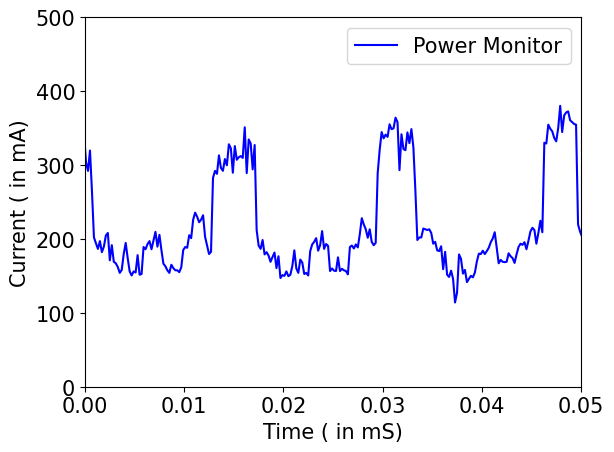
\includegraphics[width=0.50\columnwidth]{figures/candy_crush_saga_menu_timeline.png}
    \vspace{-0.1in}
    \caption{A snippet of power monitor readings for Candy Crush Saga Menu scenario on Moto Z3.}
    \label{fig:power_trace_candycrush_menu}
    \vspace{-0.2in}
\end{figure}

Second, we perform fine-grained alignment at the 1ms scale, which is
required in our feasibility study to explore SPMD at different
time scales (in \S\ref{sec:modelling_macro}--\S\ref{sec:micronano}).
The basic idea is try to match the parts of the two traces
for the same rendering interval (which has a duration of 16.7ms).
Figure~\ref{fig:power_trace_candycrush_menu} shows that
a typical rendering interval contains a GPU Busy phase followed
by a GPU Idle phase, and the Busy phase is marked
by a sharp rising edge and a sharp failing edge.
However, adjacent rendering intervals
typically have very similar power draw curves.
%  A modern smartphone on an average can generate 60 frames per second.
From the event trace we observe that the time taken to generate frames
by the GPU, \ie between two consecutive rising edges,  vary slightly, \eg
% Figure~\ref{fig:distribution_gpu_interval} shows the rendering interval spread
% for the 6 app scenarios collected from event trace.
% Our measurements shows that
the standard deviation 
for the 6 app scenarios ranges between 0.37-1.54 ms, 0.24-0.57 ms,
 and 0.10-1.42 ms,
respectively, on the 3 phones.
%   This poses a significant challenge to aligning 
%   the power monitor reading trace with the Linux event trace that we collected
%   for extracting the timings when the phone components enter different power states.
%
%   Given a power monitor trace, we mark the rising edge as the start of a
%   rendering interval and the falling edge as the end of the GPU
%   Active-busy state 
We exploit this variation in aligning the corresponding rendering intervals
in the two traces as follows.
After the coarse-grained alignment,
we choose the 50-interval window \dcomment{within 100ms offset} from the power monitor trace that has
the highest standard deviation in rendering interval durations.
%  and GPU Active-busy duration (across all of the 50 intervals).  
Next, from the event trace we use a sliding window to find the window
whose inter-GPU Busy timings best fits those of the chosen power trace window.
% 50-interval window of the power monitor trace.

% We choose a 50 interval window which we slide across 10 seconds in the middle of the trace.
% The cost function chosen is the L1-norm of the standard deviation of the total interval and
% the GPU Active-busy interval. We choose the 50 interval which has the least standard deviation.
% To align it with the event trace, we use L2 norm of the difference in the total interval
% and GPU Active-busy interval over a sliding window. 
